\documentclass[UTF8]{ctexart}
\usepackage{geometry}
\usepackage{hyperref}
\usepackage{graphicx}
\geometry{a4paper,scale=0.8}
\title{“基于朴素贝叶斯的垃圾邮件过滤算法”开题报告}
\author{150521310 何程斌}
\date{}
\begin{document}
\maketitle

\section{本题目研究的目的、意义}
随着网络技术的飞速发展,电子邮件逐渐成为人们的主要通讯工具。但是,电子邮件在给人们带来便利的同时,也带来了许多问题,其中最严重的莫过于泛滥的垃圾邮件。据Securelist(卡巴斯基实验室旗下的IT安全信息资源网站)于2017年第三季度发布的全球垃圾邮件数据显示,2017年第三季度,垃圾邮件占全球电子邮件的58.02\%,9月垃圾邮件占比最高(59.56\%)。中国是垃圾邮件的最大来源(12.24\%),前一个季度的最大来源越南的份额则下降1.2个百分点(11.17\%),排在第二位。美国排在第三位(9.62\%),印度位居第四(8.49\%)。垃圾邮件占据了网络中巨大的带宽资资源,对用户的日常工作生活带了了极大的困扰。并且,不少垃圾邮件还附带着恶意附件和网络钓鱼链接,给用户的计算机、甚至个人财产造成巨大损伤。

朴素贝叶斯分类器是一系列以假设特征之间强(朴素)独立下运用贝叶斯定理为基础的简单概率分类器,自20世纪50年代已广泛研究。在20世纪60年代初就以另外一个名称引入到文本信息检索界中\cite{ref1},并仍然是文本分类的一种热门(基准)方法,在垃圾邮件识别领域中已有了非常成熟的应用。

本文基于朴素贝叶斯算法建立一个垃圾邮件过滤器,对收集到的大量合法邮件和垃圾邮件作为样本进行有指导的学习,提取邮件的地址、主题与内容信息,建立一个有效的特征词库,从而对垃圾邮件进行高准确率的识别。


\section{国内外研究现状}
一篇英文文本转换成单词集合是很容易且精确的,因为英文的单词之间存在空格和标点这些天然分割符号。而中文博大精深,远要比英文复杂,一个字可能包含了很多种56G意思,甚至有贬有褒,是不具备独立而又有效的语义的。因此,国外的垃圾邮件分类比国内发展的迅速得多。
总体来讲,目前主要有以下几种垃圾邮件过滤技术。
\begin{enumerate}
\item 黑白名单过滤:要求收件方将经常发送垃圾邮件的域名或者 IP 放入黑名单列表中。
但当对方采用IP代理、动态 IP、地址伪造等方式发送邮件时,该方法就失效了\cite{ref2}。
\item 基于关键词:创建垃圾邮件的单词表,判断收到的邮件文本中是否存在不合法的单词,但需要一个庞大的关键词单词表\cite{ref3}。
\item 基于规则评分:通过对大量邮件的综合分析, 得到一个庞大的规则库。规则库每条规则都对应一个分数,计算邮件获得的分数,总分到达某个的阈值就会被判定为垃圾邮件。但因规则库有限,无法检测新邮件\cite{ref3})。
\item 基于内容:可分为规则角度和内容统计,用规则方法需建立完备的规则库,速度较慢。而本文所研究的基于朴素贝叶斯算法的过滤方法是一种基于内容统计的过滤方法,准确性较高\cite{ref3},并且具有很强的自我学习功能,会不断地动态调整垃圾邮件集和合法邮件集的概率。
\end{enumerate}


\section{拟采取的研究路线}
\begin{enumerate}
\item 查阅资料,学习朴素贝叶斯算法的原理,并参考课题相关的论文,研究朴素贝叶斯算法在垃圾邮件分类上的具体应用。
\item 收集邮件样本。研究垃圾邮件过滤需要大量的垃圾邮件和正常邮件数据样本,所以数据的收集、储存就是本设计的一个重要组成部分。
\item 学习 Python 语言课题相关库的使用。近年来,Python 语言来在科学计算、机器学习、自然语言处理等领域有着成熟的应用,网络上有海量的资源和成熟的第三方库,如 scikit-learn、pkuseg\cite{pkuseg}等。
\item 结合上述几个步骤所得,对本课题进行具体的实现。
\end{enumerate}


\section{进度安排}
\begin{itemize}
\item 第1-2周,资料查询,翻译英文资料,开题报告,知识准备;
\item 第3-4周,熟悉开发工具,查阅相关文档,研究程序框架;
\item 第5-6周,编写测试小程序,研究架构的合理分配;
\item 第7-8周,程序实现基于朴素贝叶斯算法的垃圾邮件过滤器;
\item 第9-12周,程序调试;
\item 第13-15周,撰写毕业论文,按要求修改;
\item 第16周,进行预答辩和程序、毕业论文的检查。
\end{itemize}

\section{文献综述}
\subsection{相关概念的定义与介绍}
\subsubsection{朴素贝叶斯(Naive Bayes)}
贝叶斯定理是概率论中的一个定理,描述在已知一些条件下,某事件的发生概率。比如,如果已知某癌症与寿命有关,使用贝叶斯定理则可以通过得知某人年龄,来更加准确地计算出他罹患癌症的概率。

朴素贝叶斯是一种十分简单的分类算法,该算法是有监督的学习算法,解决的是分类问题,如客户是否流失、是否值得投资、信用等级评定等多分类问题,其核心思想在于选择发生概率高的作为分类的结果。该算法的优点在于简单易懂、学习效率高、在某些领域的分类问题中能够与决策树、神经网络相媲美。

最为广泛的两种分类模型是决策树模型(Decision Tree Model)和朴素贝叶斯模型(Naive Bayesian Model,NBM)。和决策树模型相比,朴素贝叶斯分类器(Naive Bayes Classifier,或 NBC)发源于古典数学理论,有着坚实的数学基础,以及稳定的分类效率。同时,NBC模型所需估计的参数很少,对缺失数据不太敏感,算法也比较简单。理论上,NBC模型与其他分类方法相比具有最小的误差率。但是实际上并非总是如此,这是因为NBC模型假设属性之间相互独立,这个假设在实际应用中往往是不成立的,这给NBC模型的正确分类带来了一定影响。\cite{lihang}
\subsubsection{分词(Word Segmentation)}
分词技术就是搜索引擎针对用户提交查询的关键词串进行的查询处理后根据用户的关键词串用各种匹配方法进行的一种技术。当然,我们在进行数据挖掘、精准推荐和自然语言处理工作中也会经常用到中文分词技术。词是最小的能够独立活动的有意义的语言成分,英文单词之间是以空格作为自然分界符的,而汉语是以字为基本的书写单位,词语之间没有明显的区分标记,因此,中文词语分析是中文信息处理的基础与关键。\cite{nlp}中文分词在业界也已经有了十分成熟的工具包,如最广泛使用的 jieba,清华大学的 THULAC 等。但本研究拟使用清华大学于2019年2月开源的pkuseg。相较于其他几个工具包,pkuseg具有更高的分词准确率。根据北大研究组的测试结果,pkuseg 分别在示例数据集(MSRA 和 CTB8)上降低了 79.33\% 和 63.67\% 的分词错误率。同时,该工具包还支持多领域分词:研究组训练了多种不同领域的分词模型。根据待分词的领域特点,用户可以自由地选择不同的模型。最重要的是,该工具包还支持用户使用全新的标注数据进行训练。\cite{pkuseg}
\subsubsection{停用词(Stop Words)}
停用词是指在信息检索中,为节省存储空间和提高搜索效率,在处理自然语言数据(或文本)之前或之后会自动过滤掉某些字或词,这些字或词即被称为Stop Words(停用词)。这些停用词都是人工输入、非自动化生成的,生成后的停用词会形成一个停用词表。但是,并没有一个明确的停用词表能够适用于所有的工具。甚至有一些工具是明确地避免使用停用词来支持短语搜索的。

在基于词的检索系统中,停用词是指出现频率太高、没有太大检索意义的词,如“的、是、太、of、the”等;在基于支持向量机的自动分类中,停用词指没有实意的虚词和类别色彩不强的中性词;在自动问答系统中,停用词因其问题的不同而动态变化;在机器翻译、知识抽取中几乎没有真正的停用词,只是把频率太高的虚词作为临时的停用词特殊处理,切分完后仍然需要标记。\cite{stopwords}

本研究拟使用\url{https://github.com/goto456/stopwords},该仓库包含了中文停用词表、哈工大停用词表、百度停用词表和四川大学机器智能实验室停用词库四个常用的停用词表。将这四个停用词表作并集可以得到一个十分巨大的停用词表。
\subsubsection{混淆矩阵}
混淆矩阵是数据科学、数据分析和机器学习中总结分类模型预测结果的情形分析表,以矩阵形式将数据集中的记录按照真实的类别与分类模型作出的分类判断两个标准进行汇总。

以二元分类问题为例,数据集存在肯定类别和否定类别两类记录,而分类模型对记录分类可能作出阳性判断(判断记录属于肯定类别)或阴性判断(判断记录属于否定类别)两种判断。

混淆矩阵是一个2 × 2的情形分析表,显示以下四组记录的数目:作出正确判断的肯定记录(真阳性)、作出错误判断的肯定记录(假阴性)、作出正确判断的否定记录(真阴性)以及作出错误判断的否定记录(假阳性)。
\begin{center}
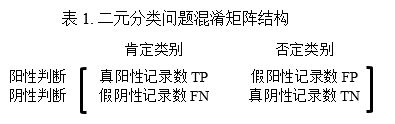
\includegraphics[scale=0.6]{pictures/v2-026440fdfe0a0a799a135cc534cb61e2_hd.jpg}
\end{center}

混淆矩阵是对分类模型进行性能评价的重要工具。由混淆矩阵可以计算真阳性率、假阳性率、真阴性率、假阴性率、准确率、精确率和F指标等各种评价指标。特别是混淆矩阵区分了假阳性和假阴性两种不同性质的误判,可以用来估计分类模型误判造成的期望损失。\cite{conmat}
\subsubsection{精确率(Precision)}
精确率(precision)定义为:$P=\frac{T P}{T P+F P}$是针对预测结果而言的,它表示的是预测为肯定类别的样本中有多少是真正的肯定类别样本
\subsubsection{召回率(Recall)}
召回率(recall)定义为:$R=\frac{T P}{T P+F N}$是针对原来的样本而言的,它表示的是样本中的肯定类别样本有多少被预测正确了。

\subsection{存在的问题与挑战}
文献中报道的召回率高达99\%或更多,有很多因素需要考虑。
\begin{enumerate}
	\item 学术研究的邮件不能代表一般的邮件,不同渠道,甚至不同时间段得到的垃圾邮件样本和正常邮件样本会有很大差别。比如Ling-Spam是语言学家之间的通信,那么语言学的术语一定在其特征向量中占很大比例。时间的因素也很重要,比如在圣诞节期间搜集的垃圾邮件,可能很大一部分都包含圣诞节,而正常邮件是关于夏季旅游的,这样就可能造成圣诞节的关键词变成垃圾邮件特征,而夏季游泳则是正常邮件特征。
	\item 目前贝叶斯方法过滤邮件的研究集中在英文邮件的处理,对于中文垃圾邮件的过滤方法和效果还有待研究。在英文等单字节字母语言中,具有独立意义的单词被空格自然分开,易于识别以进行统计。而对于中文等双字节语言来说,各个词语之间没有自然的间隔,贝叶斯分类方法就不能直接适用。
	\item 随着垃圾邮件过滤技术的进步,垃圾邮件制造者同时也在不断地适应和对付过滤器,制造出可以绕过过滤器的邮件。贝叶斯方法的本质是基于对邮件中的特征词进行统计来判别垃圾邮件。这样,垃圾邮件制造者可以通过在垃圾邮件中大量填充正常邮件的常用词,以减少垃圾邮件常用词的相对出现频率,增大正常邮件常用词相对出现频率来进行欺骗。这样,贝叶斯方法就很难识别出这个邮件。另外,把一个垃圾邮件的特征词通过HTML标记分隔开来,也可以起到绕开过滤的作用。
\end{enumerate}

\section{总结}
垃圾邮件问题已经受到了包括学者、商业界、法律界等各界人士在内的广泛关注,目前已经有专门针对该领域的多项国际会议。基于朴素贝叶斯算法的垃圾邮件过滤是解决垃圾邮件的重要方法。目前的研究主要借鉴机器学习的方法,从已有的训练语料中学习垃圾邮件的规律来指导后续邮件的判断。包括Bayes、决策树、SVM, Boosting在内的很多机器学习方法都被应用到垃圾邮件过滤中。从目前的研究结果看,这些机器学习方法在一些小规模语料上似乎可以达到实用的程度。但是,在实际应用时仍然有许多工作要做。这是因为,垃圾邮件过滤是一项长期的斗争。在我们对付垃圾邮件的同时,垃圾邮件制造者也在挖空心思制造更“合理”或者严重干扰过滤器的垃圾邮件。因此,一方面,对垃圾邮件的预处理显得越来越重要(即还原到邮件的真实内容);另一方面,垃圾邮件过滤器也要不断地更新来适应垃圾邮件的一些新特征。另外,在真正的实用垃圾邮件系统中,综合各种方法(包括各种机器学习方法、黑白名单人工规则方法甚至图片分析方法等)和各种特征(除正文内容外,还包括群发特征、元信息特征等)是垃圾邮件工具研制的趋势。

\begin{thebibliography}{99}
	\bibitem{ref1}Russell, Stuart; Norvig, Peter. Artificial Intelligence: A Modern Approach 2nd. Prentice Hall. 2003 [1995]. ISBN 978-0137903955.
	\bibitem{ref2}杨雷,曹翠玲,孙建国,张立国.改进的朴素贝叶斯算法在垃圾邮件过滤中的研究[J].通信学报,2017,38(04):140-148.
	\bibitem{ref3}张培,纪鸿旭,李璐.基于朴素贝叶斯的中文垃圾邮件过滤[J].信息与电脑(理论版),2017(07):79-81.
	\bibitem{ref4}马哲. 垃圾邮件过滤系统的研究与实现[D]. 浙江大学, 2005.
	\bibitem{pkuseg}Xu Sun, Houfeng Wang, Wenjie Li. Fast Online Training with Frequency-Adaptive Learning Rates for Chinese Word Segmentation and New Word Detection. Proceedings of ACL. 253–262. 2012
	\bibitem{nlp}李航.统计学习方法.北京:清华大学出版社,2012
	\bibitem{lihang}成庆 .统计自然语言处理(第2版).北京:清华大学出版社,2013
	\bibitem{stopwords}化柏林	. 知识抽取中的停用词处理技术[J]. 现代图书情报技术, 2007, 2(8): 48-51.	
	\bibitem{conmat}confusion matrix  .wikipedia.2019-02-04
	\bibitem{ref5}徐梦龙,黄家旺.朴素贝叶斯算法在垃圾邮件过滤方面的应用[J].网络安全技术与应用,2018(07):46-47.
	\bibitem{ref6}曹翠玲,王媛媛,袁野,赵国冬.用于垃圾邮件的贝叶斯过滤算法研究[J].网络与信息安全学报,2017,3(03):64-70.
	\bibitem{ref7}刘秋阳,林泽锋,栾青青.基于朴素贝叶斯算法的垃圾短信智能识别系统[J].电脑知识与技术,2016,12(12):190-192.
	\bibitem{ref8}张东亮,董礼.基于改进的朴素贝叶斯算法在垃圾短信过滤中的研究[J].计算机测量与控制,2012,20(02):526-528+551.
	\bibitem{ref9}周修考.基于朴素贝叶斯算法的中文垃圾邮件过滤器的设计与应用[J].兰州工业高等专科学校学报,2010,17(06):5-7.
	\bibitem{ref10}郑炜,沈文,张英鹏.基于改进朴素贝叶斯算法的垃圾邮件过滤器的研究[J].西北工业大学学报,2010,28(04):622-627.
	\bibitem{ref11}翟军昌.基于朴素贝叶斯算法的个性化垃圾邮件过滤[J].长春师范学院学报(自然科学版),2009,28(04):17-20.
	\bibitem{ref12}杨杉,何跃,颜锦江.基于贝叶斯的反垃圾邮件技术探讨[J].网络安全技术与应用,2007(08):54-56.
	\bibitem{ref13}刘宏伟,黄静.基于朴素贝叶斯算法的垃圾邮件网关[J].微计算机信息,2006(18):73-75+69.
	\bibitem{ref14}AFZAL H, MEHMOOD K. Spam filtering of bi-lingual tweets using machine learning[C]//The 18th International Conference on Advanced Communication Technology. 2016: 710- 714.
\end{thebibliography}



\end{document}
